\documentclass[12pt]{article}
\usepackage{graphicx}
\usepackage{longtable}
\begin{document}

\begin{center}
  \textbf{Amity University Punjab}
\end{center}

\begin{center}
  
\includegraphics[width=1.55625in,height=1.83333in]{media/image.png}
\end{center}

\begin{center}
  \textbf{Introduction to Cloud Computing-- {[}CSE-208{]}}

  \textbf{Assignment - II}

  \vspace{1in}

  \textbf{Submitted to:}

  Prof. Sanjay Gupta

  Amity University, Punjab\\ \\

  \vspace{1in}

  \textbf{Submitted by:}

  Gurmukh Singh

  B. Tech CSE-A (IV-Sem)

  A25305223008
\end{center}

\newpage

\textbf{1. Identify a real-world business scenario and recommend a
suitable cloud deployment model.}

\textbf{Scenario: Online Food Delivery Platform}

\textbf{Business Overview:}

A startup called \textbf{"TastyGo"} plans to launch an online food
delivery platform that connects users with local restaurants. The
platform will have a mobile app and website, support real-time order
tracking, offer discounts, and manage large volumes of user data,
payment info, and restaurant menus.

\textbf{Business Needs:}

\begin{itemize}
\item
  \textbf{Scalability:} Handle traffic spikes during meal times and
  festivals.
\item
  \textbf{High availability:} 24/7 uptime with minimal downtime.
\item
  \textbf{Cost-efficiency:} Pay-as-you-go model since the startup wants
  to manage expenses.
\item
  \textbf{Security:} Protect customer data and payment info.
\item
  \textbf{Rapid deployment:} Quickly launch updates and new features.
\end{itemize}

\textbf{Recommended Cloud Deployment Model: Public Cloud}

\textbf{Why Public Cloud is Suitable:}

\begin{itemize}
\item
  \textbf{Scalability:} Services like \textbf{AWS Elastic Beanstalk},
  \textbf{Azure App Service}, or \textbf{Google App Engine} auto-scale
  to handle more users.
\item
  \textbf{Cost-effective:} No upfront investment in infrastructure; pay
  only for resources used.
\item
  \textbf{Quick deployment:} Developers can deploy apps and updates
  quickly using CI/CD pipelines.
\item
  \textbf{Security:} Top public cloud providers offer robust security
  and compliance certifications.
\item
  \textbf{Managed services:} Reduce overhead by using managed databases
  (e.g., Amazon RDS, Firebase), load balancers, and storage (e.g.,
  Amazon S3).
\end{itemize}

\textbf{Example Implementation:}

\begin{itemize}
\item
  \textbf{Compute:} AWS EC2 or Google App Engine for running backend
  services.
\item
  \textbf{Database:} Firebase Realtime DB or Amazon RDS for
  customer/order data.
\item
  \textbf{Storage:} Amazon S3 for storing menu images and receipts.
\item
  \textbf{Analytics:} Google Analytics or AWS CloudWatch for monitoring
  usage.
\item
  % 
\includegraphics[width=3.70139in,height=3.70139in]{media/image2.jpg}\textbf{Security:}
  SSL certificates, AWS Identity and Access Management (IAM), and
  firewall settings.
\end{itemize}

\textbf{Alternative Consideration:}

If the business was a large enterprise needing \textbf{complete control
and data privacy}, a \textbf{Private Cloud} (like OpenStack) or
\textbf{Hybrid Cloud} (mix of on-premises and cloud, like using Azure
Arc) could be considered.\\
But for most \textbf{startups and SMEs}, \textbf{Public Cloud} is the
ideal choice.

\textbf{Business Scenario 2:}

"\textbf{FinSure}" is a well-established bank planning to launch a
\textbf{secure digital banking platform} offering services like savings
accounts, loans, investment tracking, credit card management, and mobile
payments. The platform is expected to serve \textbf{millions of
customers}, operate \textbf{24/7}, and store \textbf{highly sensitive
financial and personal data}.

The bank must comply with \textbf{strict regulatory standards},
including \textbf{data residency}, \textbf{PCI-DSS}, and \textbf{ISO
27001} compliance. The platform will also include \textbf{AI-driven
financial advisory services} and \textbf{custom reports for enterprise
clients}, which demand powerful computing resources but also
\textbf{tight control over data and infrastructure}.

\textbf{Business Requirements:}

\begin{itemize}
\item
  \textbf{Maximum Security:} Sensitive data such as account details,
  financial transactions, and personal information must be protected
  with \textbf{bank-level encryption and compliance protocols}.
\item
  \textbf{Regulatory Compliance:} Must follow \textbf{regional and
  international regulations} regarding data protection and financial
  reporting.
\item
  \textbf{Full Control Over Infrastructure:} The organization prefers
  complete authority over data storage, access management, and system
  updates.
\item
  \textbf{High Availability:} Services like mobile banking and card
  transactions must be \textbf{always accessible}.
\item
  \textbf{Limited Public Access:} Internal banking operations and
  customer data shouldn\textquotesingle t reside in a shared or public
  environment.
\end{itemize}

\textbf{Recommended Cloud Deployment Model: Private Cloud}

A \textbf{Private Cloud} is the most suitable option for FinSure because
it offers \textbf{dedicated infrastructure}, full customization, and
\textbf{maximum control over security and compliance}. It can be
deployed \textbf{on-premises} or through \textbf{a trusted managed
private cloud vendor}.

\textbf{Why Private Cloud is the Best Fit:}

\begin{itemize}
\item
  \textbf{High Security \& Compliance:} Private cloud allows strict
  enforcement of \textbf{security policies}, \textbf{firewalls},
  \textbf{encryption}, and \textbf{custom audit mechanisms} that public
  cloud options may not fully support.
\item
  \textbf{Dedicated Resources:} Since the infrastructure is not shared,
  there's no risk of data leakage from other tenants --- a critical
  requirement in financial services.
\item
  \textbf{Compliance-Ready Environment:} Tailored setups for
  \textbf{regulatory frameworks} such as GDPR, PCI-DSS, RBI regulations
  (India), and others.
\item
  \textbf{Custom Architecture:} The IT team can design, monitor, and
  update the infrastructure to suit internal security and operational
  protocols.
\item
  \textbf{Predictable Performance:} As resources aren't shared with
  others, \textbf{latency is lower}, and performance is consistent.
\end{itemize}

\textbf{Example Cloud Setup for FinSure:}

\begin{longtable}[]{@{}
  >{\raggedright\arraybackslash}p{(\columnwidth - 2\tabcolsep) * \real{0.2140}}
  >{\raggedright\arraybackslash}p{(\columnwidth - 2\tabcolsep) * \real{0.7860}}@{}}
\toprule\noalign{}
\begin{minipage}[b]{\linewidth}\raggedright
Component
\end{minipage} & \begin{minipage}[b]{\linewidth}\raggedright
Private Cloud Option
\end{minipage} \\
\midrule\noalign{}
\endhead
\bottomrule\noalign{}
\endlastfoot
Infrastructure & Hosted via VMware vSphere or OpenStack in on-prem data
centre \\
Database & Private SQL cluster for transaction records and customer
data \\
Storage & Encrypted SAN/NAS storage with role-based access control \\
Security & Custom firewalls, DLP systems, intrusion detection, audit
trails \\
Backup \& DR & Private replication and recovery systems in secondary
data centres \\
\end{longtable}

\textbf{2. Classify different organizations based on which cloud model
they should use.}

\textbf{1. Entertainment \& Streaming Organizations → Public Cloud}

\textbf{Recommended Model:} Public Cloud

\textbf{Why:}

\begin{itemize}
\item
  These organizations cater to millions of users globally.
\item
  They require on-demand scalability to handle sudden traffic surges
  (e.g., new show releases).
\item
  Public cloud offers global content delivery, low latency, and cost
  efficiency.
\end{itemize}

\textbf{Examples:}

\begin{itemize}
\item
  Netflix uses AWS to deliver streaming services to over 190 countries.
\item
  Spotify relies on Google Cloud Platform to process real-time music
  data, recommendations, and analytics.
\item
  Disney+ scales rapidly on AWS during new releases like Marvel or Star
  Wars shows.
\end{itemize}

\textbf{2. Banking \& Financial Institutions → Private Cloud}

\textbf{Recommended Model:} Private Cloud

\textbf{Why:}

\begin{itemize}
\item
  Banks deal with highly sensitive data like personal, transactional,
  and credit card information.
\item
  They must comply with financial regulations (e.g., PCI-DSS, RBI
  Guidelines).
\item
  Private clouds give them maximum security, control, and customization
  options.
\end{itemize}

\textbf{Examples:}

\begin{itemize}
\item
  Bank of America uses a private cloud for secured financial
  transactions and compliance.
\item
  JP Morgan Chase maintains internal cloud systems for real-time risk
  analysis and data security.
\item
  HDFC Bank (India) uses private cloud infrastructure to support its
  digital banking services securely.
\end{itemize}

\textbf{3. Retail \& E-Commerce Companies → Hybrid Cloud}

\textbf{Recommended Model:} Hybrid Cloud

\textbf{Why:}

\begin{itemize}
\item
  Retailers need to process customer data, orders, inventory, and run
  large-scale websites/apps.
\item
  Hybrid cloud lets them store critical data privately while using the
  public cloud to manage high web traffic or sales peaks.
\item
  It also allows integration with legacy systems while adopting modern
  cloud tools.
\end{itemize}

\textbf{Examples:}

\begin{itemize}
\item
  Walmart uses a hybrid model: private cloud for internal operations,
  Azure for customer-facing apps.
\item
  Flipkart leverages a hybrid approach to run AI-based recommendations
  while managing supply chains securely.
\item
  Amazon itself uses hybrid setups for combining warehouse systems and
  AWS.
\end{itemize}

\textbf{4. Government, Research \& Defence Organizations → Private or
Community Cloud}

\textbf{Recommended Model: Private or Community Cloud}

\textbf{Why:}

\begin{itemize}
\item
  These bodies handle classified or confidential information like
  national security data or scientific research.
\item
  Private cloud offers tight control and security; community cloud
  allows collaboration between departments under shared rules.
\item
  Government agencies often have regulatory restrictions on where data
  can be stored.
\end{itemize}

\textbf{Examples:}

\begin{itemize}
\item
  NASA uses the Nebula private cloud for secure and high-performance
  computing in space research.
\item
  ISRO (India) uses secured infrastructure for handling space mission
  data, satellite communication, etc.
\item
  EU Government Agencies use community cloud to securely share
  information across departments while staying compliant with GDPR.
\end{itemize}

\textbf{5. Healthcare Providers → Hybrid or Community Cloud}

\textbf{Recommended Model:} Hybrid / Community Cloud

\textbf{Why:}

\begin{itemize}
\item
  Healthcare systems must store electronic health records (EHRs) and
  patient data with privacy (HIPAA, etc.).
\item
  Community clouds help hospitals share data securely while meeting
  common compliance.
\item
  Hybrid clouds allow sensitive data to remain private while leveraging
  public cloud for applications, analytics, or appointment booking
  systems.
\end{itemize}

\textbf{Examples:}

\begin{itemize}
\item
  NHS UK uses a community cloud to allow hospitals to securely access
  and update patient records.
\item
  Mayo Clinic (USA) partners with Google Cloud to provide AI-driven
  diagnostics and secure research collaboration.
\item
  Apollo Hospitals use hybrid cloud for secure storage of patient data
  and running their health apps.
\end{itemize}

\textbf{6. Educational Institutions \& Universities → Community Cloud}

\textbf{Recommended Model:} Community Cloud

\textbf{Why:}

\begin{itemize}
\item
  Universities and research institutes often collaborate across borders
  on shared scientific research, labs, and academic resources.
\item
  Community cloud allows them to share infrastructure and data securely,
  while keeping costs low.
\item
  It supports access control, data sharing, and joint platforms for
  learning and discovery.
\end{itemize}

\textbf{Examples:}

\begin{itemize}
\item
  CERN operates a community cloud to support research on particle
  physics involving institutions worldwide.
\item
  Open Science Data Cloud (OSDC) enables researchers to store and share
  massive scientific datasets.
\item
  IITs/NITs (India) use platforms provided by NIC and shared research
  clouds to collaborate nationally and internationally.
\end{itemize}

% 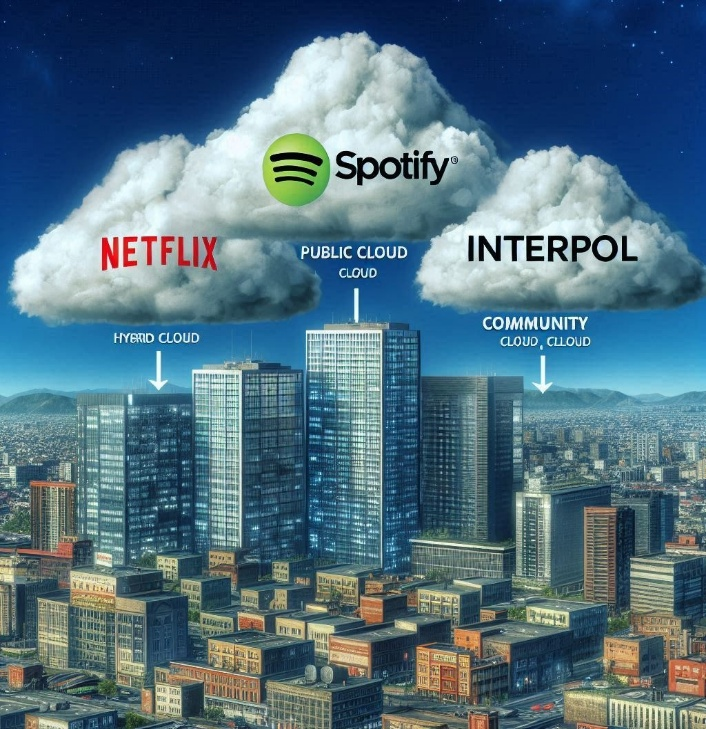
\includegraphics[width=3.20833in,height=3.3125in]{media/image3.jpeg}

\textbf{3. Compare and contrast different cloud deployment models based
on cost, security, and scalability.}

Cloud deployment models define how cloud infrastructure is structured,
accessed, and managed. Choosing the right model depends on several
business needs including budget, sensitivity of data, compliance
requirements, and growth potential.

\textbf{Public Cloud}

\begin{itemize}
\item
  Operated by third-party providers like Amazon Web Services (AWS),
  Microsoft Azure, or Google Cloud Platform (GCP).
\item
  Resources like servers and storage are shared among multiple
  organizations, making it very cost-efficient.
\item
  Ideal for startups and growing businesses looking to avoid upfront
  infrastructure costs.
\item
  While public cloud providers offer strong baseline security,
  organizations have limited control over data management, making it
  less suitable for sensitive information.
\end{itemize}

\begin{quote}
\textbf{Private Cloud}
\end{quote}

\begin{itemize}
\item
  The cloud infrastructure is dedicated to a single organization, hosted
  either on-premises or through a private third-party provider.
\item
  Offers maximum security and data privacy, making it the best option
  for industries dealing with confidential or regulated data such as
  banking, defense, or healthcare.
\item
  Since the infrastructure is not shared, the cost of setup and
  maintenance is significantly higher, but control over performance and
  compliance is unparalleled.
\item
  Scalability depends on the organization's own IT capabilities or
  hosting arrangements.
\end{itemize}

\begin{quote}
\textbf{Hybrid Cloud}
\end{quote}

\begin{itemize}
\item
  Combines features of both public and private clouds, allowing
  businesses to store sensitive data in a secure private cloud while
  leveraging the public cloud for high-volume or less critical
  operations.
\item
  Provides a flexible and balanced solution --- organizations can
  optimize for cost, performance, and compliance.
\item
  Ideal for enterprises with mixed workloads, seasonal demands, or those
  undergoing digital transformation.
\item
  Highly scalable due to public cloud integration, while maintaining
  control over sensitive functions.
\end{itemize}

\begin{quote}
\textbf{Community Cloud}
\end{quote}

\begin{itemize}
\item
  A cloud environment shared by a group of organizations that have
  similar security, compliance, or operational concerns (e.g.,
  hospitals, universities, government departments).
\item
  Infrastructure is jointly owned and managed, offering customized
  compliance, cost-sharing, and secure collaboration.
\item
  More affordable than private cloud and more secure than public cloud,
  making it suitable for domain-specific use cases.
\item
  Commonly used in sectors like healthcare (e.g., NHS UK), education,
  and scientific research consortia.
\end{itemize}

\begin{quote}
\textbf{Comparison Table :}
\end{quote}

\begin{longtable}[]{@{}
  >{\raggedright\arraybackslash}p{(\columnwidth - 10\tabcolsep) * \real{0.1867}}
  >{\raggedright\arraybackslash}p{(\columnwidth - 10\tabcolsep) * \real{0.1509}}
  >{\raggedright\arraybackslash}p{(\columnwidth - 10\tabcolsep) * \real{0.1766}}
  >{\raggedright\arraybackslash}p{(\columnwidth - 10\tabcolsep) * \real{0.1549}}
  >{\raggedright\arraybackslash}p{(\columnwidth - 10\tabcolsep) * \real{0.1500}}
  >{\raggedright\arraybackslash}p{(\columnwidth - 10\tabcolsep) * \real{0.1810}}@{}}
\toprule\noalign{}
\begin{minipage}[b]{\linewidth}\raggedright
\begin{quote}
Deployment Model
\end{quote}
\end{minipage} & \begin{minipage}[b]{\linewidth}\raggedright
\begin{quote}
Cost
\end{quote}
\end{minipage} & \begin{minipage}[b]{\linewidth}\raggedright
\begin{quote}
Security
\end{quote}
\end{minipage} & \begin{minipage}[b]{\linewidth}\raggedright
\begin{quote}
Scalability
\end{quote}
\end{minipage} & \begin{minipage}[b]{\linewidth}\raggedright
\begin{quote}
Real-World Example
\end{quote}
\end{minipage} & \begin{minipage}[b]{\linewidth}\raggedright
\begin{quote}
Best Suited For
\end{quote}
\end{minipage} \\
\midrule\noalign{}
\endhead
\bottomrule\noalign{}
\endlastfoot
\end{longtable}

\begin{longtable}[]{@{}
  >{\raggedright\arraybackslash}p{(\columnwidth - 10\tabcolsep) * \real{0.1876}}
  >{\raggedright\arraybackslash}p{(\columnwidth - 10\tabcolsep) * \real{0.1750}}
  >{\raggedright\arraybackslash}p{(\columnwidth - 10\tabcolsep) * \real{0.1750}}
  >{\raggedright\arraybackslash}p{(\columnwidth - 10\tabcolsep) * \real{0.1375}}
  >{\raggedright\arraybackslash}p{(\columnwidth - 10\tabcolsep) * \real{0.1625}}
  >{\raggedright\arraybackslash}p{(\columnwidth - 10\tabcolsep) * \real{0.1624}}@{}}
\toprule\noalign{}
\begin{minipage}[b]{\linewidth}\raggedright
\begin{quote}
Public Cloud
\end{quote}
\end{minipage} & \begin{minipage}[b]{\linewidth}\raggedright
\begin{quote}
Low (Pay-as-you-go; no upfront infra investment)
\end{quote}
\end{minipage} & \begin{minipage}[b]{\linewidth}\raggedright
\begin{quote}
Moderate -- Vendor-managed security in shared environment
\end{quote}
\end{minipage} & \begin{minipage}[b]{\linewidth}\raggedright
\begin{quote}
Very High -- Scales instantly on demand
\end{quote}
\end{minipage} & \begin{minipage}[b]{\linewidth}\raggedright
\begin{quote}
Netflix (video streaming on AWS)
\end{quote}
\end{minipage} & \begin{minipage}[b]{\linewidth}\raggedright
\begin{quote}
Startups, E-commerce, SaaS platforms
\end{quote}
\end{minipage} \\
\midrule\noalign{}
\endhead
\bottomrule\noalign{}
\endlastfoot
\end{longtable}

\begin{longtable}[]{@{}
  >{\raggedright\arraybackslash}p{(\columnwidth - 10\tabcolsep) * \real{0.1876}}
  >{\raggedright\arraybackslash}p{(\columnwidth - 10\tabcolsep) * \real{0.1750}}
  >{\raggedright\arraybackslash}p{(\columnwidth - 10\tabcolsep) * \real{0.1754}}
  >{\raggedright\arraybackslash}p{(\columnwidth - 10\tabcolsep) * \real{0.1377}}
  >{\raggedright\arraybackslash}p{(\columnwidth - 10\tabcolsep) * \real{0.1619}}
  >{\raggedright\arraybackslash}p{(\columnwidth - 10\tabcolsep) * \real{0.1624}}@{}}
\toprule\noalign{}
\begin{minipage}[b]{\linewidth}\raggedright
\begin{quote}
Private Cloud
\end{quote}
\end{minipage} & \begin{minipage}[b]{\linewidth}\raggedright
\begin{quote}
High (Dedicated hardware and management)
\end{quote}
\end{minipage} & \begin{minipage}[b]{\linewidth}\raggedright
\begin{quote}
Very High -- Full control over data and compliance
\end{quote}
\end{minipage} & \begin{minipage}[b]{\linewidth}\raggedright
\begin{quote}
Moderate -- Limited to internal resources unless vendor-hosted
\end{quote}
\end{minipage} & \begin{minipage}[b]{\linewidth}\raggedright
\begin{quote}
Bank of America (secure financial systems)
\end{quote}
\end{minipage} & \begin{minipage}[b]{\linewidth}\raggedright
\begin{quote}
Banks, Governments, Defence, Large Enterprises
\end{quote}
\end{minipage} \\
\midrule\noalign{}
\endhead
\bottomrule\noalign{}
\endlastfoot
\end{longtable}

\begin{longtable}[]{@{}
  >{\raggedright\arraybackslash}p{(\columnwidth - 10\tabcolsep) * \real{0.1876}}
  >{\raggedright\arraybackslash}p{(\columnwidth - 10\tabcolsep) * \real{0.1750}}
  >{\raggedright\arraybackslash}p{(\columnwidth - 10\tabcolsep) * \real{0.1750}}
  >{\raggedright\arraybackslash}p{(\columnwidth - 10\tabcolsep) * \real{0.1375}}
  >{\raggedright\arraybackslash}p{(\columnwidth - 10\tabcolsep) * \real{0.1625}}
  >{\raggedright\arraybackslash}p{(\columnwidth - 10\tabcolsep) * \real{0.1624}}@{}}
\toprule\noalign{}
\begin{minipage}[b]{\linewidth}\raggedright
\begin{quote}
Hybrid Cloud
\end{quote}
\end{minipage} & \begin{minipage}[b]{\linewidth}\raggedright
\begin{quote}
Moderate (Optimized use of public and private)
\end{quote}
\end{minipage} & \begin{minipage}[b]{\linewidth}\raggedright
\begin{quote}
High -- Sensitive operations in private, bulk workloads in public
\end{quote}
\end{minipage} & \begin{minipage}[b]{\linewidth}\raggedright
\begin{quote}
Very High Leverages elasticity of public cloud
\end{quote}
\end{minipage} & \begin{minipage}[b]{\linewidth}\raggedright
\begin{quote}
Walmart (retail apps on hybrid cloud)
\end{quote}
\end{minipage} & \begin{minipage}[b]{\linewidth}\raggedright
\begin{quote}
Enterprises with variable workloads or scaling needs
\end{quote}
\end{minipage} \\
\midrule\noalign{}
\endhead
\bottomrule\noalign{}
\endlastfoot
\end{longtable}

\begin{longtable}[]{@{}
  >{\raggedright\arraybackslash}p{(\columnwidth - 10\tabcolsep) * \real{0.1896}}
  >{\raggedright\arraybackslash}p{(\columnwidth - 10\tabcolsep) * \real{0.1750}}
  >{\raggedright\arraybackslash}p{(\columnwidth - 10\tabcolsep) * \real{0.1750}}
  >{\raggedright\arraybackslash}p{(\columnwidth - 10\tabcolsep) * \real{0.1375}}
  >{\raggedright\arraybackslash}p{(\columnwidth - 10\tabcolsep) * \real{0.1625}}
  >{\raggedright\arraybackslash}p{(\columnwidth - 10\tabcolsep) * \real{0.1604}}@{}}
\toprule\noalign{}
\begin{minipage}[b]{\linewidth}\raggedright
\begin{quote}
Community Cloud
\end{quote}
\end{minipage} & \begin{minipage}[b]{\linewidth}\raggedright
\begin{quote}
Moderate (Cost shared among participants)
\end{quote}
\end{minipage} & \begin{minipage}[b]{\linewidth}\raggedright
\begin{quote}
High -- Tailored security \& regulatory compliance for the group
\end{quote}
\end{minipage} & \begin{minipage}[b]{\linewidth}\raggedright
\begin{quote}
Moderate to High Depends on collective growth
\end{quote}
\end{minipage} & \begin{minipage}[b]{\linewidth}\raggedright
\begin{quote}
NHS UK (healthcare data collaboration)
\end{quote}
\end{minipage} & \begin{minipage}[b]{\linewidth}\raggedright
\begin{quote}
Healthcare alliances, Universities, Research clusters
\end{quote}
\end{minipage} \\
\midrule\noalign{}
\endhead
\bottomrule\noalign{}
\endlastfoot
\end{longtable}

\textbf{4. What factors influence the choice of a cloud deployment model
for a business?}

\textbf{1. Data Sensitivity and Security Requirements}

\begin{quote}
\textbf{What it Means:}

If a business deals with highly confidential data---like financial
transactions, defence operations, patient records---it cannot risk
exposing this data to the public. In such cases, businesses often prefer
Private or Community Clouds.

\textbf{Use Case:}
\end{quote}

\begin{itemize}
\item
  Industries like banking, healthcare, defence, and legal services
  prioritize data encryption, internal access control, and audit
  capabilities.
\end{itemize}

\begin{quote}
\textbf{Real Example:}
\end{quote}

\begin{itemize}
\item
  JP Morgan Chase uses a Private Cloud to store sensitive financial
  data, ensuring it\textquotesingle s not exposed to any third-party
  public infrastructure.
\item
  ISRO stores satellite and mission data in its private infrastructure
  to ensure national security.
\end{itemize}

\textbf{2. Compliance and Regulatory Requirements}

\begin{quote}
\textbf{What it Means:}

Many industries must comply with laws such as:
\end{quote}

\begin{itemize}
\item
  HIPAA (healthcare),
\item
  GDPR (EU data privacy),
\item
  PCI-DSS (financial data security), which dictate how and where data
  must be stored and processed.
\end{itemize}

\begin{quote}
\textbf{Use Case:}
\end{quote}

\begin{itemize}
\item
  Businesses often choose Private or Community Clouds to meet specific
  legal compliance standards and local data residency requirements.
\end{itemize}

\begin{quote}
\textbf{Real Example:}
\end{quote}

\begin{itemize}
\item
  NHS UK uses a Community Cloud to meet healthcare-specific legal
  frameworks and ensures all patient data remains within the UK.
\item
  EU government agencies operate on a community cloud that respects GDPR
  and allows controlled data sharing across departments.
\end{itemize}

\textbf{3. Budget and Cost Constraints}

\begin{quote}
\textbf{What it Means:}

Small to medium-sized businesses or startups often lack large capital
for hardware and infrastructure. They look for flexible and
cost-effective solutions where they pay only for what they use.

\textbf{Use Case:}
\end{quote}

\begin{itemize}
\item
  The Public Cloud is the go-to model here, offering scalability with
  minimal upfront investment and no maintenance responsibility.
\end{itemize}

\begin{quote}
\textbf{Real Example:}
\end{quote}

\begin{itemize}
\item
  Zomato, during its early growth phase, used AWS (Public Cloud) to host
  their services. This allowed them to scale as demand increased without
  investing heavily in physical infrastructure.
\end{itemize}

\textbf{4. Scalability Needs}

\begin{quote}
\textbf{What it Means:}

Some businesses experience fluctuating workloads---for instance, during
peak shopping seasons or major product launches. These businesses
require infrastructure that can scale up or down instantly.

\textbf{Use Case:}
\end{quote}

\begin{itemize}
\item
  Public or Hybrid Cloud offers elastic scalability, making it ideal for
  businesses that deal with variable demand or rapid growth.
\end{itemize}

\begin{quote}
\textbf{Real Example:}
\end{quote}

\begin{itemize}
\item
  Netflix uses AWS (Public Cloud) to automatically scale during peak
  viewing times (e.g., global premieres) to serve millions of concurrent
  users without performance loss.
\end{itemize}

\textbf{5. Control Over Infrastructure}

\begin{quote}
\textbf{What it Means:}

Organizations with complex internal systems or unique hardware/software
needs may require custom configurations, tight security controls, or
dedicated resources.

\textbf{Use Case:}
\end{quote}

\begin{itemize}
\item
  Private Cloud allows full control over the infrastructure---ideal for
  organizations that cannot risk using a shared environment.
\end{itemize}

\begin{quote}
\textbf{Real Example:}
\end{quote}

\begin{itemize}
\item
  NASA uses a Private Cloud (Nebula) where all systems are configured to
  support space research, simulation, and data analysis with zero
  external access.
\end{itemize}

\textbf{6. Nature of Workload or Application}

\begin{quote}
\textbf{What it Means:}

Depending on whether an application is customer-facing (e.g., mobile
apps, websites) or internal (e.g., payroll, CRM), the cloud deployment
model may vary.

\textbf{Use Case:}
\end{quote}

\begin{itemize}
\item
  Businesses may use Public Cloud for public-facing services and Private
  Cloud for sensitive internal operations. Hybrid Cloud combines both.
\end{itemize}

\begin{quote}
\textbf{Real Example:}
\end{quote}

\begin{itemize}
\item
  Walmart hosts internal systems like inventory and HR in a Private
  Cloud, while using Public Cloud to manage its online store and mobile
  app traffic.
\end{itemize}

\textbf{7. Collaboration and Shared Purpose}

\begin{quote}
\textbf{What it Means:}

Organizations that collaborate on shared goals (like research or
education) can benefit from a Community Cloud, which provides a secure
and cost-effective shared environment.

\textbf{Use Case:}
\end{quote}

\begin{itemize}
\item
  Multiple institutions working on joint research, academic programs, or
  public services can pool resources without compromising security.
\end{itemize}

\begin{quote}
\textbf{Real Example:}
\end{quote}

\begin{itemize}
\item
  CERN uses a Community Cloud to enable physicists and institutions
  worldwide to analyse data from the Large Hadron Collider
  collaboratively.
\end{itemize}

\textbf{8. Legacy System Integration}

\begin{quote}
\textbf{What it Means:}

Large enterprises with old on-premise infrastructure may find it
difficult to move entirely to the cloud. Instead, they gradually
modernize by combining on-prem with cloud services using a Hybrid Cloud.

\textbf{Use Case:}
\end{quote}

\begin{itemize}
\item
  Hybrid Cloud allows smooth transition and integration without shutting
  down mission-critical legacy systems.
\end{itemize}

\begin{quote}
\textbf{Real Example:}
\end{quote}

\begin{itemize}
\item
  General Electric (GE) uses a Hybrid Cloud strategy to modernize its
  industrial operations while continuing to support existing on-site
  systems.
\end{itemize}

\textbf{5. Identify a scenario where a community cloud would be the most
suitable deployment model.}

\textbf{Scenario: Inter-Governmental Data Sharing}

\textbf{Use Case:}

Several government agencies---like the \textbf{Police Department},
\textbf{Customs}, and \textbf{Tax Authorities}---need to:

\begin{itemize}
\item
  Share sensitive information (like criminal records or financial
  audits)
\item
  Follow \textbf{common security policies and legal frameworks}
\item
  Maintain \textbf{data sovereignty} (must store data within the
  country/region)
\item
  % \includegraphics[width=4.05in,height=4.05in]{media/image4.jpg}Have
  \textbf{cost-effective} infrastructure shared across departments
\end{itemize}

\textbf{Why Community Cloud?}

\begin{itemize}
\item
  \textbf{Shared infrastructure} lowers costs for all participating
  agencies
\item
  Built with \textbf{common compliance standards} (e.g., GDPR, CJIS,
  etc.)
\item
  Allows \textbf{secure collaboration} without exposing data to
  outsiders
\item
  Offers better \textbf{control} than public cloud but more
  \textbf{affordability} than private cloud
\end{itemize}

\textbf{Real-World Example:}

\textbf{European Union (EU) Government Cloud}

Several EU departments use a \textbf{Community Cloud model} for:

\begin{itemize}
\item
  Law enforcement collaboration
\item
  Judicial and tax data sharing
\item
  Ensuring compliance with \textbf{EU data protection regulations
  (GDPR)}
\end{itemize}

Managed by trusted entities, with \textbf{common governance policies}

\textbf{Other Possible Use Cases:}

\begin{itemize}
\item
  \textbf{Universities} sharing research data (e.g., CERN)
\item
  \textbf{Healthcare networks} sharing patient records under common laws
  (e.g., NHS trusts in the UK)
\item
  \textbf{Financial cooperatives} maintaining shared ledgers and risk
  assessment tools
\end{itemize}

\begin{quote}
\textbf{Scenario: Collaborative Healthcare Network Using Community
Cloud}

\textbf{Overview}
\end{quote}

In modern healthcare systems, it is essential for multiple
entities---such as \textbf{hospitals, clinics, diagnostic labs,
pharmacies}, and \textbf{government health departments}---to work
together to provide high-quality, coordinated care. This requires
\textbf{seamless, secure, and efficient sharing of data}, which includes
sensitive patient records, test results, prescriptions, and treatment
plans.

However, due to the \textbf{highly sensitive nature of medical data},
healthcare institutions must comply with strict regulations such as
\textbf{HIPAA (Health Insurance Portability and Accountability Act)} in
the United States, or \textbf{NDHM (National Digital Health Mission)} in
India. This makes it difficult to use public cloud solutions where
control is minimal and data is often stored in multi-tenant
environments.

\textbf{Why Community Cloud is Ideal for This Scenario}

A \textbf{Community Cloud} is designed to support a \textbf{specific
group of organizations with shared concerns} such as compliance,
performance, and security. In this case, the healthcare industry
benefits from a shared infrastructure that caters specifically to their
needs:

\begin{quote}
\textbf{1. Shared Purpose and Governance}

All participating healthcare institutions have \textbf{common goals}:
improving patient outcomes, reducing delays in care, and promoting
health research. The cloud environment is jointly governed by these
stakeholders, ensuring policies and operations align with medical
standards.

\textbf{2. Regulatory Compliance}

A Community Cloud can be \textbf{custom-built to comply with healthcare
regulations}. This ensures that \textbf{electronic health records
(EHRs)} and patient information remain secure and private, while being
accessible to authorized personnel only.

\textbf{3. Secure and Controlled Access}

Only authorized members of the healthcare community can access the
cloud, making it \textbf{more secure than public cloud} models. Access
control policies, encryption, and data auditing features are implemented
according to the needs of the healthcare sector.

\textbf{4. Cost Efficiency through Resource Sharing}

Instead of each hospital maintaining its own expensive IT
infrastructure, costs are \textbf{shared among all members}, reducing
financial burden while still enjoying high-end cloud capabilities.

\textbf{5. Real-Time Collaboration}
\end{quote}

Doctors, labs, and pharmacies can \textbf{access real-time patient
data}, track medical history, and coordinate treatments more
effectively, which is especially valuable during emergencies or
outbreaks.

\textbf{Real-World Example: NHS (National Health Service), UK}

The NHS in the United Kingdom uses a \textbf{Community Cloud
infrastructure} to:

\begin{itemize}
\item
  \textbf{Securely store and share patient data} between hospitals,
  clinics, and general practitioners.
\item
  Ensure \textbf{compliance with the UK Data Protection Act} and
  healthcare regulations.
\item
  Promote \textbf{efficiency, cost savings}, and better patient outcomes
  through shared digital platforms.
\end{itemize}

\textbf{Additional Example: Academic Research Collaborations}

A group of universities working on \textbf{climate change research} can
benefit from a Community Cloud where they:

\begin{itemize}
\item
  Share large datasets like satellite imagery and weather models.
\item
  Use common tools for analysis while keeping \textbf{research data
  secure and isolated} from the public.
\item
  Reduce costs by \textbf{sharing computing power} and storage
  infrastructure.
\end{itemize}

\textbf{Conclusion :}

A \textbf{Community Cloud} is the most suitable deployment model when:

\begin{itemize}
\item
  Multiple organizations need to \textbf{collaborate on sensitive data}.
\item
  There is a \textbf{shared interest} in security, compliance, and
  efficiency.
\item
  The group wants to \textbf{balance control with cost-effectiveness}.
\end{itemize}
\end{document}
